\documentclass{article}
\usepackage[utf8]{inputenc}

\title{CSE 222A PROJECT - GROUP 6}

\author{Sreejith Unnikrishnan, Stanislav Mushits, Amit Borase, Ritvik Jaiswal }
\date{November 4 2015}

\usepackage{natbib}
\usepackage{graphicx}

\begin{document}

\maketitle

\begin{center}
\textbf{Milestone report}
\end{center}


\section{Project Topic}
We are working towards verification of varys scheduler\cite{varys} and associated performance improvement in a data center environment. As a part of this goal, we have completed the following tasks.

\section{Setting up Virtual Machines}
The first step we performed was to setup the allotted virtual machine. We analyzed the required programming environment, tools and dependencies. Based on the analysis we ensured that the required programs and API`s are installed on the machine. A shell script was written to automate this task, under utils directory of our repository. This makes the process of adding a new VM to our setup easier.

\section{Deciding the network topology}
Datacenter environment is unique in terms of traffic patterns and topology and because of that we gave special care while designing our network topology. Given that the topology will affect the data transmission efficiency of different coflows, we decided to work on a fat-tree based network setup. It consists of hosts, edge switches, aggregation layer switches and core switches. We use the open source library 'Fast Network Simulation Setup (FNSS)' \cite{fnss} for topology development, which then later on is used to deploy mininets. We made sure that the important topology parameters can be easily configured and the software structure is flexible enough to accommodate future changes.

\section{Topology development}
We created topology generator code using Python, namely topo\_gen.py \cite{repo}, using the FNSS framework. The topology generator requires 'network.config' file as an input. It parses the file to get the K value for fat-tree topology, the link speeds, link delay etc. By changing these values we can simulate different network environments as required without altering the code. Once the topology is created using FNSS, we port the topology into an XML file, so that it could be reused by other programs. We then convert the FNSS topology into mininet topology which can be deployed in the VM. Finally we ensure all the hosts are working by doing a ping test.

\section{Tracefile generator}


\section{Trace segregator}
Network traces thus generated consists of event schedules for all the network hosts (mappers and reducers bith) in a single big XML dataset. To be able to schedule this traffic individually, we need to segregate it into per network hosts dataset. We achieved this by writing a python based segregator that parses and writes XML data to individual host's network traces.

\section{Host programs and controller}
For conducting network simulation we built a program which  operates on each host. This program (called Actor) accept during launch:
\begin{itemize}
\item configuration file which helps synchronize all hosts for starting in the same time and contain simulation parameters
\item file with tasks which should be executed during simulation.
\item After launch Actor synchronizes with other hosts and start simulation.
\item It has two modes of simulation:

\begin{itemize}
\item traditional simulation, which uses regular flows
\item Vary's simulation, which uses coflows
\end{itemize}
\end{itemize}

For each simulation type Actor takes each task and execute it according to simulation type, sending amount of data specified by task to another host.
For now, it executes all tasks sequentially and opens new connection for each new task. In future, the program will be updated to 

\begin{itemize}
\item open one connection for each Reducer and hold it till finishing of MapReduce
\item send data in parallel
\item log all actions and give them back for analysis
\end{itemize}

\section{System structure}
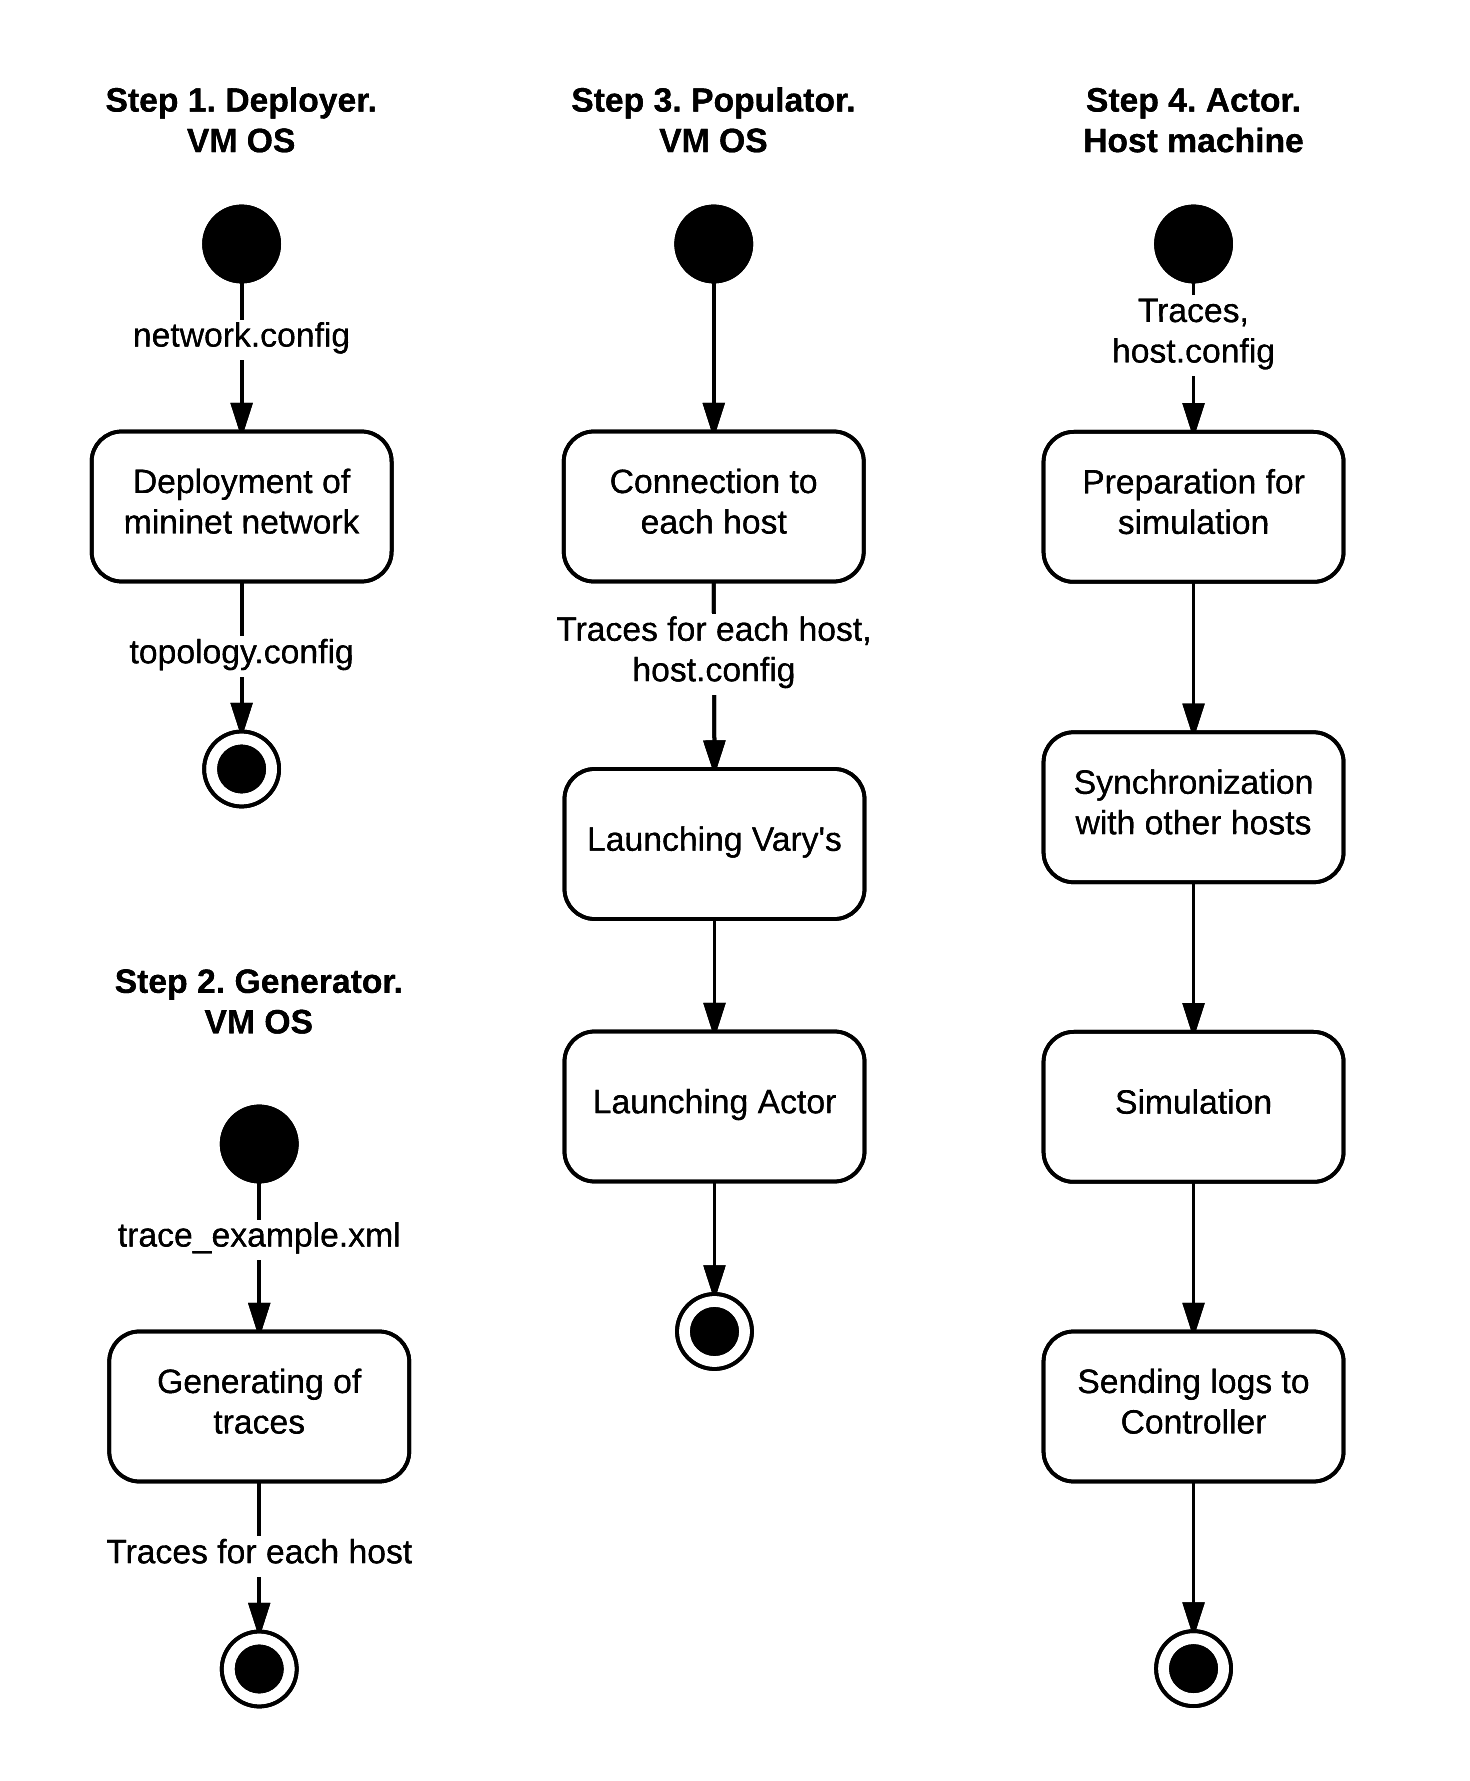
\includegraphics[scale = 0.75]{flow_diagram}
\begin{itemize}
\item The deployer program takes network.config file and creates the required topology.
\item The trace generator generates trace files for each host
\item The populator program in the VM host launches varys in each hosts and launches actor program
\item The actor machine gathers trace file, host config and run the simulation. The results are logged
\end{itemize}

\section{Challenges faced}
One of the main challenges was to design the proper and efficient topology that simulates a datacenter network. To make our simulation more realistic, we studied different papers regarding datacenter networks, the ones discussed during classes and beyond that. We decided on fat tree topology since it is widely used at the moment and provides efficient bisection bandwidth for all the hosts. We found an open source tool FNSS, written at University College of London, which provides effective API`s to model fat tree topology for data centers. We used the FNSS API to generate the topology. However we need to run Varys scheduler in each of the hosts. That means we would have to go with mininet. So in our program we generate the topology with FNSS and then convert it to Mininet.

The next task is to model and generate Map reduce traffic. To understand the traffic pattern we read through many papers including the Facebook paper written by Prof. Porter \cite{facebook}, which helped understand fundamental differences between web traffic pattern and map reduce jobs. We created a trace file in accordance with our study results and we are planning to use the same for our future.

Once we ensured we have the proper information regarding data traffic to be generated, our next job was to work on the system architecture. This was also a challenging task since the code should be simple, flexible for future changes and simulate the data center environment accurately. We ensured the design was modular and all the important parameters configurable.

\section{Graphs}
We will be reporting the following graphs after the experiments
\begin{itemize}
\item Compatison of coflow completion times with and without varys scheduler for map reduce traffic. We evaluate whether coflow scheduler improves the performance of such traffic patterns. X axis will have the Coflow completion time while y axis will contain the factor of improvement.
\item Comparison of coflow completion times with varying coflow sizes, with and without varys scheduler running. X axis will contain the coflow completion times for different coflow sizes and y axis plots the improvement factor with and without varys scheduler.
\end{itemize}

\section{Next steps}

The next steps we are planning to complete are as follows,

\begin{itemize}
\item Integrate individual parts to bring up the system
\item Using a simple test verify that the setup is up and running
\item Run the test with proper data using varys scheduler
\item Run similar test with hosts not running varys scheduler
\item Measure and compare the results
\end{itemize}

\bibliographystyle{plain}
\begin{thebibliography}{10}
\bibitem{varys}
Efficient Coflow Scheduling with Varys, Mosharaf Chowdhury, Yuan Zhong, Ion Stoica, ACM SIGCOMM, 2014.

\bibitem{fnss}
Fast Network Simulation Setup \textit{https://github.com/fnss/fnss/}

\bibitem{repo}
Team 06 Github Repo \textit{https://github.com/ucsdcse222a/group6}

\bibitem{facebook}
Inside the Social Network’s (Datacenter) Network - SIGCOMM 2015
\textit{Arjun Roy, Hongyi Zeng, Jasmeet Bagga, George Porter, and Alex C. Snoeren}

\end{thebibliography}

\end{document}
